\documentclass[handout]{ximera}

\input{../preamble}

\outcome{Create and apply the distance formula in three dimensions.}

\title{1.1 Distance in Space}



\begin{document}

\begin{abstract}
In this section we create the distance formula in space and apply it to spheres.
\end{abstract}

\maketitle


\section{One Dimension}

The real number line, denoted $\R$ (or $\R^1$ for emphasis) consists of all real numbers.  In interval notation, we can write $\R = (-\infty, \infty)$.
The distance between two real numbers $x_1$ and $x_2$ is given by $d = |x_2 - x_1|$. Note that $d = 0$ if and only if $x_1 = x_2$.


\begin{center}
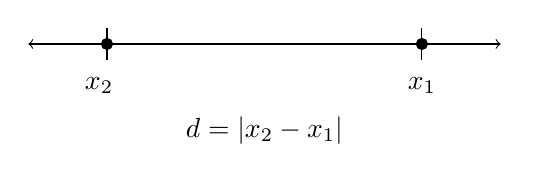
\begin{tikzpicture}
\draw[<->] (-3,0) -- (3,0) node[right]{$\R$};
\draw (-2,-.2) -- (-2,.2); %tick mark
\draw (2,-.2) -- (2,.2);
\draw[fill] (-2,0) circle [radius=0.07];
\draw[fill] (2,0) circle [radius=0.07];
\node[below] at (-2.1,-.3) {$x_2$};
\node[below] at (2,-.3) {$x_1$};
\node[below] at (0,-.8) {$d = |x_2 - x_1|$};
\end{tikzpicture}
\end{center}

\begin{example}[Example 1]
Show that the points $-3$ and $6$ in $\R^1$ are equidistant to the point $1.5$.\\
Let $d_1$ be the distance from $-3$ to $1.5$ and let $d_2$ be the distance from $6$ to $1.5$. Then
\[
d_1 = |-3 - 1.5| = |-4.5| = 4.5
\]
and
\[
d_2 = |6 - 1.5| = |4.5| = 4.5
\]
Since $d_1 = d_2$, the points $-3$ and $6$ are equidistant to $1.5$ in $\R^1$.
\end{example}

\begin{problem}(Problem 1)
Use the distance formula in $\R^1$ to verify that the midpoint between the real numbers $x_1$ and $x_2$ is 
\[
\text{midpoint} = \frac{x_1 +x_2}{2}
\]
\begin{hint}
You may assume that $x_1 < x_2$
\end{hint}

\begin{hint}
Compute the distances from $x_1$ and $x_2$ from the supposed midpoint
\end{hint}
\end{problem}


Here is a video solution of problem 1:\\
\begin{foldable}
\youtube{4CdR9fxSxkM}
\end{foldable}


\section{Two Dimensions}
Two-dimensional Euclidean space, $\R^2$, is typically represented geometrically by the $xy$-plane. 
In formal terms, $\R^2$ is the set of all coordinate pairs of real numbers:
 \[
\R^2 = \{(x,y) \,|\, x, y \in \R\}
\]

The distance formula in $\R^2$ comes from the Pythagorean Theorem. If $(x_1, y_1)$ and $(x_2, y_2)$ are points in $\R^2$, then from the triangle below,
we can see that the distance between them is given by 
\[
d = \sqrt{(x_2 - x_1)^2 + (y_2 - y_1)^2}
\]






In two dimensions, we used slopes to verify that the midpoint was actually on the line segment connecting the endpoints.  
To accomplish this in three dimensions, we need to use vectors.
\end{document}



